%% Template for a preprint Letter or Article for submission
%% to the journal Nature.
%%

\documentclass[%
%superscriptaddress,
%groupedaddress,
%unsortedaddress,
%runinaddress,
%frontmatterverbose, 
%preprint,
showpacs,
%preprintnumbers,
%nofootinbib,
%nobibnotes,
%bibnotes,
 amsmath,amssymb,
 aps,
 twocolumn,
 prl,
 reprint,
%pra,
%prb,
%rmp,
%prstab,
%prstper,
floatfix,
]{revtex4-1}

\usepackage{graphicx}% Include figure files
\usepackage{dcolumn}% Align table columns on decimal point
\usepackage{bm}% bold math
%\usepackage{lineno}
\usepackage{amsmath}
\usepackage{amsfonts}
\usepackage{amssymb}
\usepackage{color}
\usepackage{acronym}
\usepackage{multirow}
\usepackage{tabularx}
\usepackage{hyperref}
%\usepackage{booktabs}

\hypersetup{
%--- fill inside borders ---
  colorlinks=true,        % false: boxed links; true: colored links
  linkcolor=black,         % color of internal links
  citecolor=cyan,         % color of links to bibliography
}

%% ----- comment commands for each of us
\newcommand{\chris}[1]{\textbf{\textcolor{red}{CHRIS: #1}}}
\newcommand{\francesco}[1]{\textbf{\textcolor{green}{FRANCESCO: #1}}}
\newcommand{\hunter}[1]{\textbf{\textcolor{blue}{HUNTER: #1}}}
\newcommand{\siong}[1]{\textbf{\textcolor{cyan}{SIONG: #1}}}
\newcommand{\rod}[1]{\textbf{\textcolor{yellow}{ROD: #1}}}

\begin{document}

\preprint{APS/123-QED}

\title{Estimating Bayesian parameter estimation using conditional variational
autoencoders for gravitational-wave astronomy}

\author{Hunter Gabbard$^1$}
 \email{Corresponding author: h.gabbard.1@research.gla.ac.uk}
\author{Chris Messenger$^1$}
\author{Ik Siong Heng$^1$}
\author{Francesco Tonolini$^2$}
\author{Roderick Murray-Smith$^2$}

\affiliation{
 SUPA, School of Physics and Astronomy$^1$, \\
 University of Glasgow, \\
 Glasgow G12 8QQ, United Kingdom \\ \\
 School of Computing Science$^2$, \\
 University of Glasgow, \\
 Glasgow G12 8QQ, United Kingdom \\
}

\date{\today}

\maketitle

% TO-DO LIST
%
% 1. Get abstract word count roughly correct - currently 195 (done)
% 2. Get total word count roughly correct - currently (195, 680, 960, 620) =
% 2455
% 3. Clean captions and check word count (done)
% 4. Fix all plots (done)
% 5. Tidy Methods section (done)
% 6. Polish language throughout (done)
% 7. Check acronyms for consistency
% 8. Check names and variables for consistency (KL, VItamin, etc...)
% 9. Fix references - check limit
% 10. Maybe change title
% 11. Maybe add extra plots to methods section
% 12. Do a spell check (done)
% 13. Fix acknowledgments (done)
% 14. Clean codes and add ref to github

\acrodef{GW}[GW]{Gravitational wave}
\acrodef{BBH}[BBH]{binary black hole}
\acrodef{EM}[EM]{electromagnetic}
\acrodef{CBC}[CBC]{compact binary coalescence}
\acrodef{BNS}[BNS]{binary neutron star}
\acrodef{NSBH}[NSBH]{neutron star black hole}
\acrodef{PSD}[PSD]{power spectral density}
\acrodef{ELBO}[ELBO]{evidence lower bound}
\acrodef{LIGO}[LIGO]{advanced Laser Interferometer Gravitational wave Observatory}
\acrodef{CVAE}[CVAE]{conditional variational autoencoder}
\acrodef{KL}[KL]{Kullback--§Leibler}
\acrodef{GPU}[GPU]{graphics processing unit}
\acrodef{LVC}[LVC]{LIGO-Virgo Collaboration}
\acrodef{PP}[p-p]{probability-probability}

%
% Introductory paragraph describing the content of the letter
%
% This format begins with a title of, at most, 15 words, followed by an
% introductory paragraph (not abstract) of approximately 150 words, summarizing
% the background, rationale, main results (introduced by "Here we show" or some
% equivalent phrase) and implications of the study. This paragraph should be
% referenced, as in Nature style, and should be considered part of the main
% text, so that any subsequent introductory material avoids too much redundancy
% with the introductory paragraph.
%
\textbf{ 
%
% background
%
\ac{GW} detection is now commonplace~\cite{PhysRevLett.116.061102,
PhysRevX.6.041015,PhysRevLett.119.161101} and as the sensitivity of the global
network of \ac{GW} detectors improves, we will observe $\mathcal{O}(100)$s of
transient \ac{GW} events per year~\cite{1409.7215}. For each of these events
the current methods used to estimate their source parameters employ optimally
sensitive~\cite{2009CQGra..26o5017S} but computationally costly Bayesian inference
approaches~\cite{1409.7215}.
%
% rationale
%
For \ac{BBH} signals, existing \ac{GW} analyses can take $\mathcal{O}(10^{5} -
10^{6})$ seconds to complete~\cite{1409.7215} and for \ac{BNS}
signals this increases by at least an order of magnitude
~\cite{PhysRevLett.119.161101}. It is for this latter class of signal (and
\ac{NSBH} systems) that counterpart \ac{EM} signatures are expected, containing
prompt emission on timescales of 1 second -- 1 minute. The current fastest
method for alerting \ac{EM} follow-up observers~\cite{2016PhRvD..93b4013S}, can
provide estimates in $\mathcal{O}(1)$ minute, on a limited range of key source
parameters. 
%
% results
%
Here we show that a \ac{CVAE}~\cite{1904.06264,1812.04405} pre-trained on
\ac{BBH} signals and without being given the precomputed posteriors can return
Bayesian posterior probability estimates on source parameters. The training
procedure need only be performed once for a given prior parameter space (or
signal class) and the resulting trained machine can then generate samples
describing the posterior distribution $\sim 7$ orders of magnitude faster than
existing techniques.}
%
% currently ~240 words - needs cutting to ~150
% approx 9.6 words per line

%%%%%%%%%%%%%%%%%%%%%%%%%%%%%%%%%%%%%%%%%%%%%%%%%%%%%%%%%%%%%%%%%%%%%%
% INTRODUCTION
%%%%%%%%%%%%%%%%%%%%%%%%%%%%%%%%%%%%%%%%%%%%%%%%%%%%%%%%%%%%%%%%%%%%%%
%
% introduction - this section has to expand upon what has mentioned in the
% abstract background (which was only ~50 words). It needs to cover the state of
% the gravitational wave field and the number of detections expected in the next
% ~5 years. It should briefly discuss the issue of low latency EM follow up. It
% needs to cover Bayesian inference (not in too much detail) and the signal model
% we are interested in here (again, not too much detail but enough for the
% average Nature reader). It then needs to introduce machine learning and focus
% mainly on how our scheme works. We also need to include a statement about how
% the training data priors affect the result (are they really the priors?)
%
% Intro to the detection era with the LVC
%
%With the overwhelmingly successful observation runs of O1 and O2 now complete,
%\ac{LIGO} and Virgo have produced a large catalogue of \ac{GW} data covering
%both \ac{BBH} and \ac{BNS} signals~\cite{1811.12907}. Over the next five years
%we expect the number of detections to increase to be upwards of $\sim180$
%\ac{BNS} and $\sim400$ BBH events per year~\cite{1304.0670,1811.12907}. This
%large influx in the number of detections will put an increased amount of
%pressure on the current \ac{GW} inference methods used for parameter
%estimation.  

%
% From GW detection, to parameter estimation
%
The problem of detecting \acp{GW} has largely been solved through the use of
template based matched-filtering~\cite{0264-9381-33-21-215004}, a process
recently replicated using machine learning
techniques~\cite{GEORGE201864,PhysRevLett.120.141103,GebKilParHarSch}. Once a
\ac{GW} has been identified through this process, Bayesian inference, known to
be the optimal approach~\cite{2009CQGra..26o5017S}, is used to extract
information about the source parameters of the detected \ac{GW} signal.

%
% Set up parameter estimation problem
%
In the standard Bayesian \ac{GW} inference approach, we assume a signal and
noise model and both may have unknown parameters that we are either interested
in inferring or prefer to marginalise away. Each parameter is given a prior
astrophysically motivated probability distribution and in the \ac{GW} case, we
typically assume a Gaussian additive noise model (in reality, the data is not
truly Gaussian). Given a noisy \ac{GW} waveform, we would like to find an
optimal procedure for inferring some set of the unknown \ac{GW} parameters.
Such a procedure should be able to give us an accurate estimate of the
parameters of our observed signal, whilst accounting for the uncertainty
arising from the noise in the data.

%
% Describe Bayes Theorem
%
According to Bayes' Theorem, a posterior probability distribution on a set of
parameters, conditional on the measured data, can be represented as
%
\begin{align}\label{eq:bayes_theorem} 
p(x|y) &\propto p(y|x) p(x), 
\end{align}
%
where $x$ are the parameters, $y$ is the observed data, $p(x|y)$ is the
posterior, $p(y|x)$ is the likelihood, and $p(x)$ is the prior on the
parameters. The constant of proportionality, which we omit here, is
$p(y)$, the probability of our data, known as the Bayesian evidence or the
marginal likelihood. We typically ignore $p(y)$ since it is a constant and for
parameter estimation purposes we are only interested in the shape of the
posterior.

%
% brief statement on the sampling algorithms
%
Due to the size of the parameter space typically encountered in \ac{GW}
parameter estimation and the volume of data analysed, we must stochastically
sample the parameter space in order to estimate the posterior.  Sampling is
done using a variety of techniques including Nested
Sampling~\cite{skilling2006,cpnest,dynesty} and Markov chain Monte Carlo
methods~\cite{emcee,ptemcee}. The primary software tools used by the \ac{LIGO}
parameter estimation analysis are \texttt{LALInference} and
\texttt{Bilby}~\cite{1409.7215,1811.02042}, which offer multiple sampling
methods.  
  
%
% Intro to machine learning section
%
Machine learning has featured prominently in many areas of gravitational wave
research over the last few years. These techniques have shown to be
particularly promising in signal detection
\cite{GEORGE201864,PhysRevLett.120.141103,1904.08693}, glitch classification
\cite{1706.07446,0264-9381-34-6-064003} and earthquake prediction
\cite{Coughlin_2017}. Recently, a type of neural network known as \ac{CVAE} was
shown to perform exceptionally well when applied towards computational imaging
inference~\cite{1904.06264,NIPS2015_5775}, text to image
inference~\cite{1512.00570}, high-resolution synthetic image
generation~\cite{1612.00005} and the fitting of incomplete heterogeneous
data~\cite{1807.03653}. It is this type of machine learning network that we
apply in the \ac{GW} case to accurately approximate the Bayesian posterior
$p(x|y)$.

%
% Brief introduction to loss functions used in the neural networks
%
The construction of a \ac{CVAE} begins with the definition of a quantity to be
minimised (referred to as a cost function). We can relate that aim to
that of approximating the posterior distribution by minimising the cross
entropy, defined as
%
\begin{align}\label{eq:cross_ent} 
H(p,r) &= -\int dx\, p(x|y) \log r_{\theta}(x|y) 
\end{align}
%
between the true posterior $p(x|y)$ and $r_{\theta}(x|y)$, the parametric
distribution that we will use neural networks to construct and which we aim to
be equal to the true posterior. In this case $\theta$ represents a set of
trainable neural network parameters. Starting from this point it is possible to
derive a computable form for the cross-entropy that is reliant on a set of
unknown functions that can be modelled by variational encoder
and decoder neural networks. The details of the derivation are described in
the methods section and in~\cite{1904.06264}. The final form of the
cross-entropy loss function is given by the bound
%
\begin{align}\label{eq:cost3}
H \lesssim -\frac{1}{N}\sum_{n=1}^{N}&\Big[\log
r_{\theta_{2}}(x_{n}|z_{n},y_{n})\nonumber\\
&-\text{KL}\left[q_{\phi}(z|x_{n},y_{n})||r_{\theta_{1}}(z|y_{n})\right]\Big],
\end{align}
%
and requires three fully-connected networks; two encoder networks (labelled
$\textrm{E}_1$, $\textrm{E}_2$ in Fig.~\ref{fig:network_config}) representing
the functions $r_{\theta_{1}}(z|y)$ and $q_{\phi}(z|x,y)$ respectively, and one
decoder network (D) representing the function $r_{\theta_{2}}(x|z,y)$. The
function $\text{KL}(\cdot||\cdot)$ denotes the \ac{KL} divergence and
the variable $z$ represents locations within the \emph{latent space}.  This
latter object is typically a lower dimensional space within which the encoder
networks attempt to represent their input data. In practice, during the
training procedure the various integrations that are part of the derivation are
approximated by a sum over a batch of $N$ training data samples (indexed by $n$
above) at each stage of training. Training is performed via a series of steps
detailed in the methods section.

\begin{figure}
    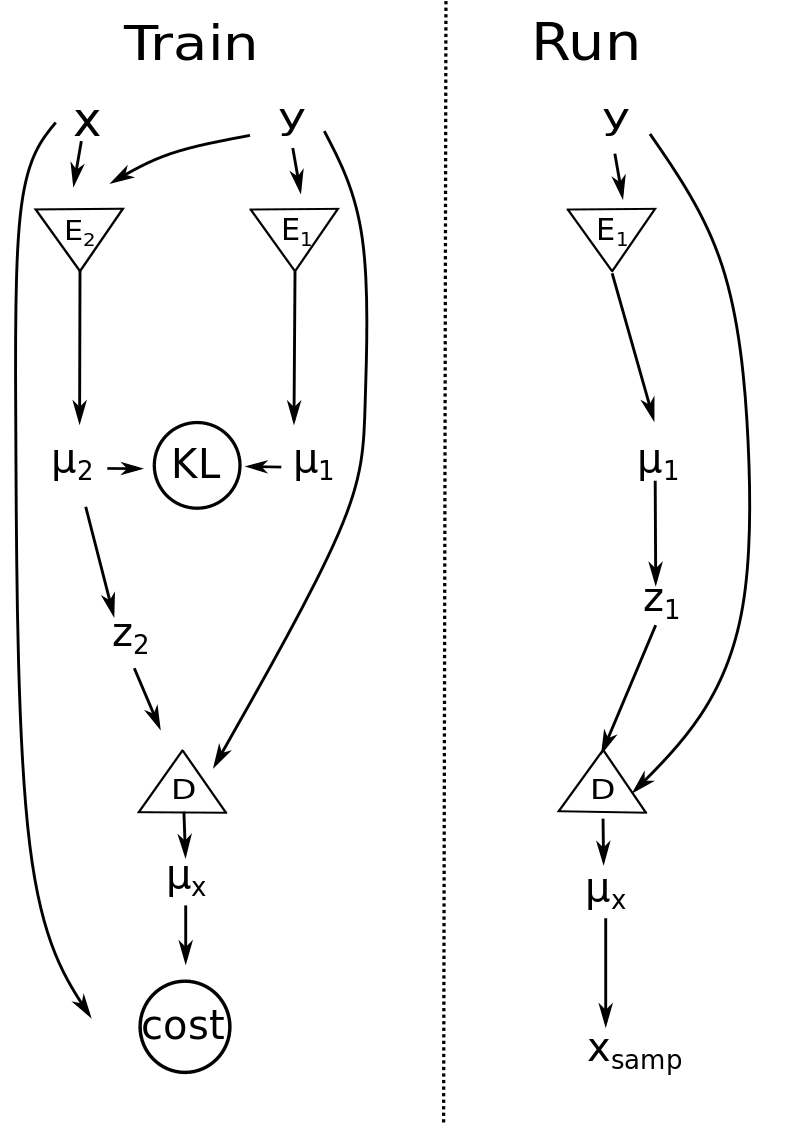
\includegraphics[width=\columnwidth]{images/network_setup.png}
    \caption{\label{fig:network_config} The configuration of the \ac{CVAE}
neural network. During training (left-hand side), a training set of noisy
\ac{GW} signals ($y$) and their corresponding true parameters ($x$) are given
as input to encoder network $\textrm{E}_2$, while only $y$ is given to
$\textrm{E}_1$.  The K-L divergence (Eq.~\ref{eq:kl}) is computed between the
encoder output latent space representations (defined by $\mu_q$ and $\mu_r$)
forming one component of the total cost function.  Samples ($z_q$) from the
$\text{E}_{2}$ latent space representation are generated and passed to the
decoder network D together with the original input data $y$. The output of the
decoder ($\mu_x$) describes a distribution in the physical space and the
\ac{ELBO} cost component $L$ is computed by evaluating that distribution at the
value of the original input $x$. When performed in batches this scheme allows
the computation of the total cost function Eq.~\ref{eq:cost3}. After having
trained the network, we test (right-hand side) using only the $\textrm{E}_1$
encoder and the decoder D to produce samples ($x_{\text{samp}}$) from the
posterior $p(x|y)$.}
\end{figure}

%
% word count ~1500 - approx 9 words per line
%

%%%%%%%%%%%%%%%%%%%%%%%%%%%%%%%%%%%%%%%%%%%%%%%%%%%%%%%%%%%%%%%%%%%%%%
% RESULTS
%%%%%%%%%%%%%%%%%%%%%%%%%%%%%%%%%%%%%%%%%%%%%%%%%%%%%%%%%%%%%%%%%%%%%%
%
% results - here you would outline the process of comparison between the
% standard approach and the new one. Define training and test data and how Bilby
% is run on all test data for comparison. How do we then train our network. How
% do we then produce results on the test data. Here you refer to results plots
% but try to not make conclusion statements (just descriptive). Also include the
% speed analysis here.
%
%
% Intro to the results - what are we trying to do?
%
We present results on $256$ single detector \ac{GW} test \ac{BBH} waveforms in
simulated advanced detector noise~\cite{aligo_noisecurves} and compare between
variants of the existing Bayesian approaches and the \ac{CVAE}. Posteriors
produced by the \texttt{Bilby} inference library~\cite{1811.02042} are used as
a benchmark in order to assess the efficiency and quality of our machine
learning approach with the existing method for posterior sampling.

%
% describe the Bilby analysis 
%
For the benchmark analysis we assume that 5 parameters are unknown: the
component masses $m_1,m_2$, the luminosity distance $d_{\text{L}}$, the time of
coalescence $t_{0}$, and the phase at coalescence $\phi_0$. For each
parameter we use a uniform prior with ranges and fixed values defined in
Table~\ref{tab:prior_ranges}.
%~\chris{we might want to
%change this to be a $d$-squared prior to demonstrate the application of priors
%in the \texttt{VItamin} training stage.} 
We use a sampling frequency of $256$~Hz and a timeseries duration of 1 second.
The waveform model used is \texttt{IMRPhenomPv2}~\cite{1809.10113} with a
minimum cutoff frequency of $20$Hz. For each input test waveform we run the
benchmark analysis using multiple sampling algorithms available within
\texttt{Bilby}. For each run and sampler we extract $3000$ samples from the
posterior on the 5 physical parameters.  

%
% the VItamin process
%
The \ac{CVAE} training process used as input $10^{6}$ waveforms corresponding
to parameters drawn from the same priors as assumed for the benchmark analysis.
The waveforms are also of identical duration, sampling frequency, and waveform
model as used in the benchmark analysis. When each waveform is placed within a
training batch it is given a unique detector noise realisation after which the
data is whitened using the same advanced detector
\ac{PSD}~\cite{2016LRR....19....1A} from which the simulated noise is
generated\footnote{Although we whiten the data as input to our network the
whitening is simply to scale the input to a level more suitable to neural
networks and need not be performed with the true \ac{PSD}.}. The \ac{CVAE}
posterior results are produced by passing our $256$ whitened noisy testing set
of \ac{GW} waveforms as input into the testing path of the pre-trained
\ac{CVAE}~\ref{fig:network_config}. For each input waveform we sample until we
have generated $3000$ posterior samples on 4 physical parameters
($x=(m_1,m_2,d_{\text{L}},t_{0})$). We choose to output a subset of the full
5-dimensional space to demonstrate that parameters (such as $\phi_0$ in this
case) can (if desired) be marginalized out within the \ac{CVAE} procedure
itself, rather than after training. 

%
% 1-D overlap results
%
\begin{figure*}
    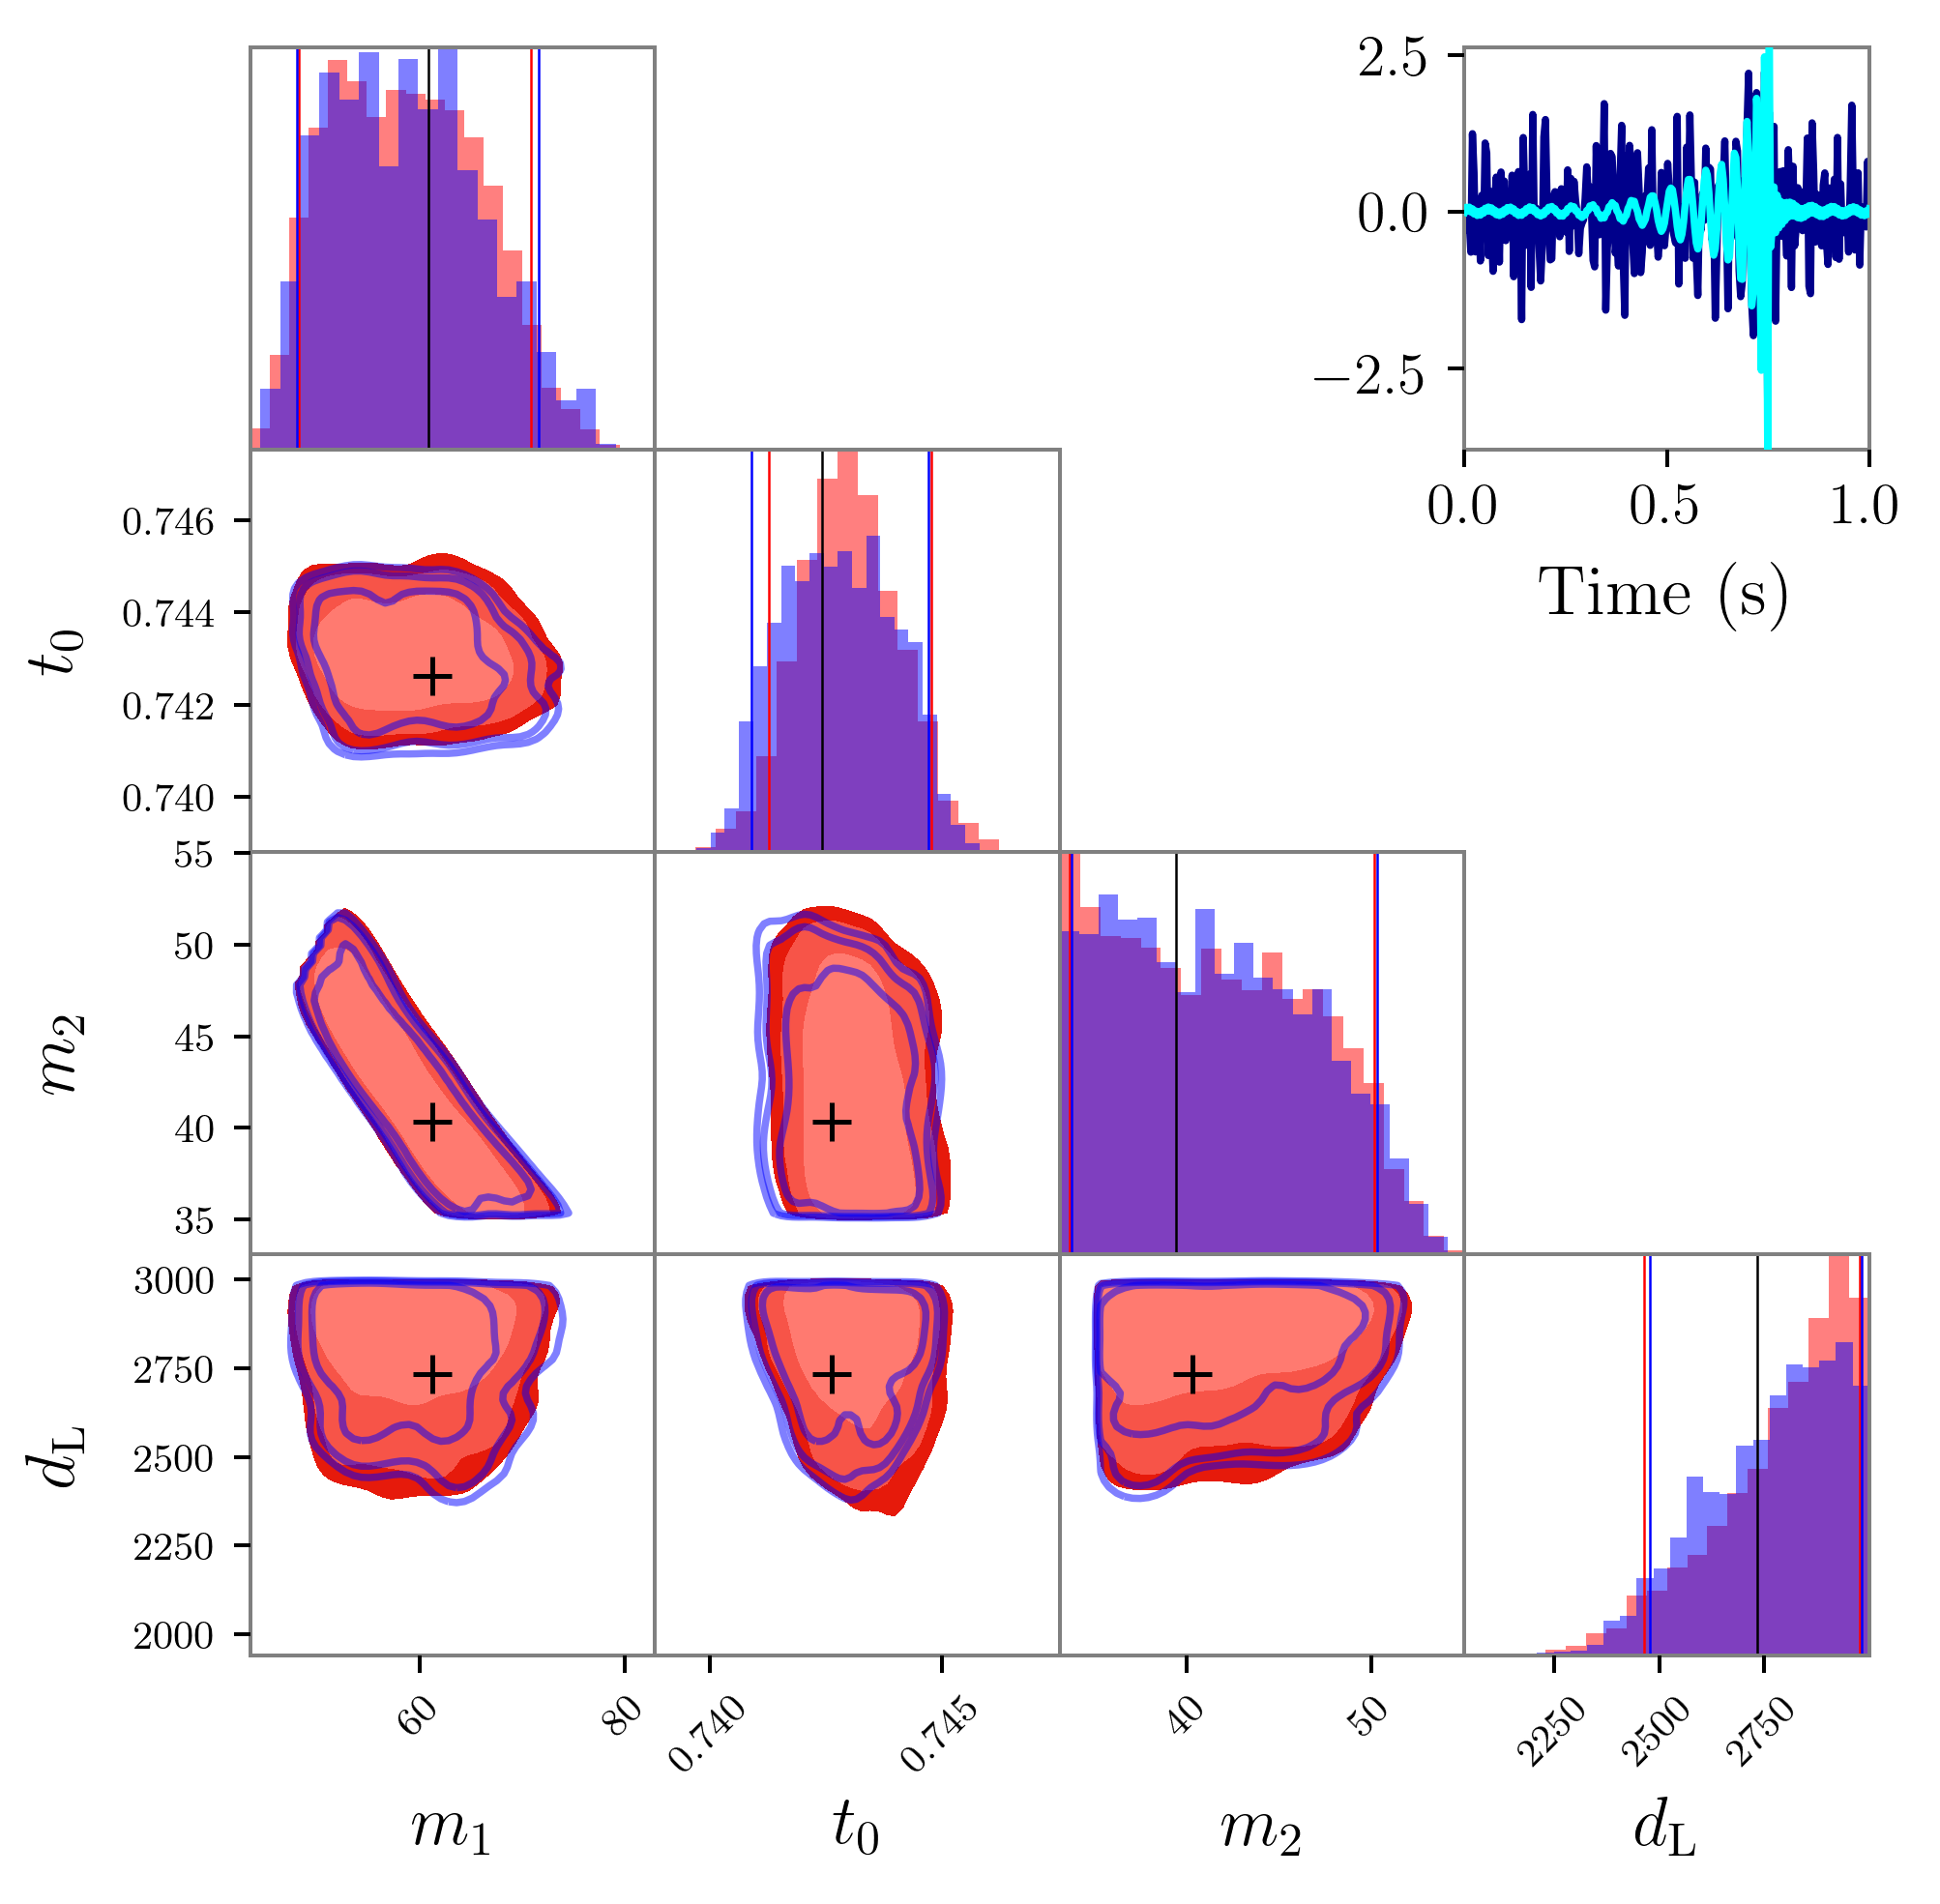
\includegraphics[width=\textwidth]{images/corner_testcase0.png}
    \caption{\label{fig:corner_plot} Corner plot showing 2 and 1-dimensional
marginalised posterior distributions for one example test dataset. Filled (red)
contours represent the posteriors obtained from the \ac{CVAE} approach and
solid (blue) contours are the posteriors output from our baseline analysis
(\texttt{Bilby} using the dynesty sampler). In each case, the contour boundaries
enclose $68,90$ and $95\%$ probability. One dimensional histograms of the
posterior distribution for each parameter from both methods are plotted along
the diagonal. Blue and red vertical lines represent the $5$---$95\%$ symmetric
confidence bounds for \texttt{Bilby} and variational inference respectively.
Black crosses and vertical black lines denote the true parameter values of the
simulated signal. The original whitened noisy timeseries $y$ and the noise-free
signal are plotted in blue and cyan respectively in the upper right hand
panel. The test signal was simulated with optimal signal-to-noise ratio of
13.9.}
\end{figure*}

%
% discuss the corner plot results
%
We can immediately illustrate the accuracy of our machine learning predictions
by directly plotting 2 and 1-dimensional marginalised posteriors generated
using the output samples from our \ac{CVAE} and \texttt{Bilby} approaches
superimposed on each other. We show this for one example test dataset in
Fig.~\ref{fig:corner_plot} where the strong agreement between both
\texttt{Bilby} (blue) and the \ac{CVAE} (red) is clear. 

%We provide additional test case example corner plots in the methods
%section. 
%\hunter{Add more corner plots in methods
%section}~\chris{Maybe, but more corner plots aren't going to convince people.
%We need to agregate the results into a single figure somehow (like the KL
%values). I think something based on the 1-D intervals would be nice.}

%
% P-P plot
%
\begin{figure}
    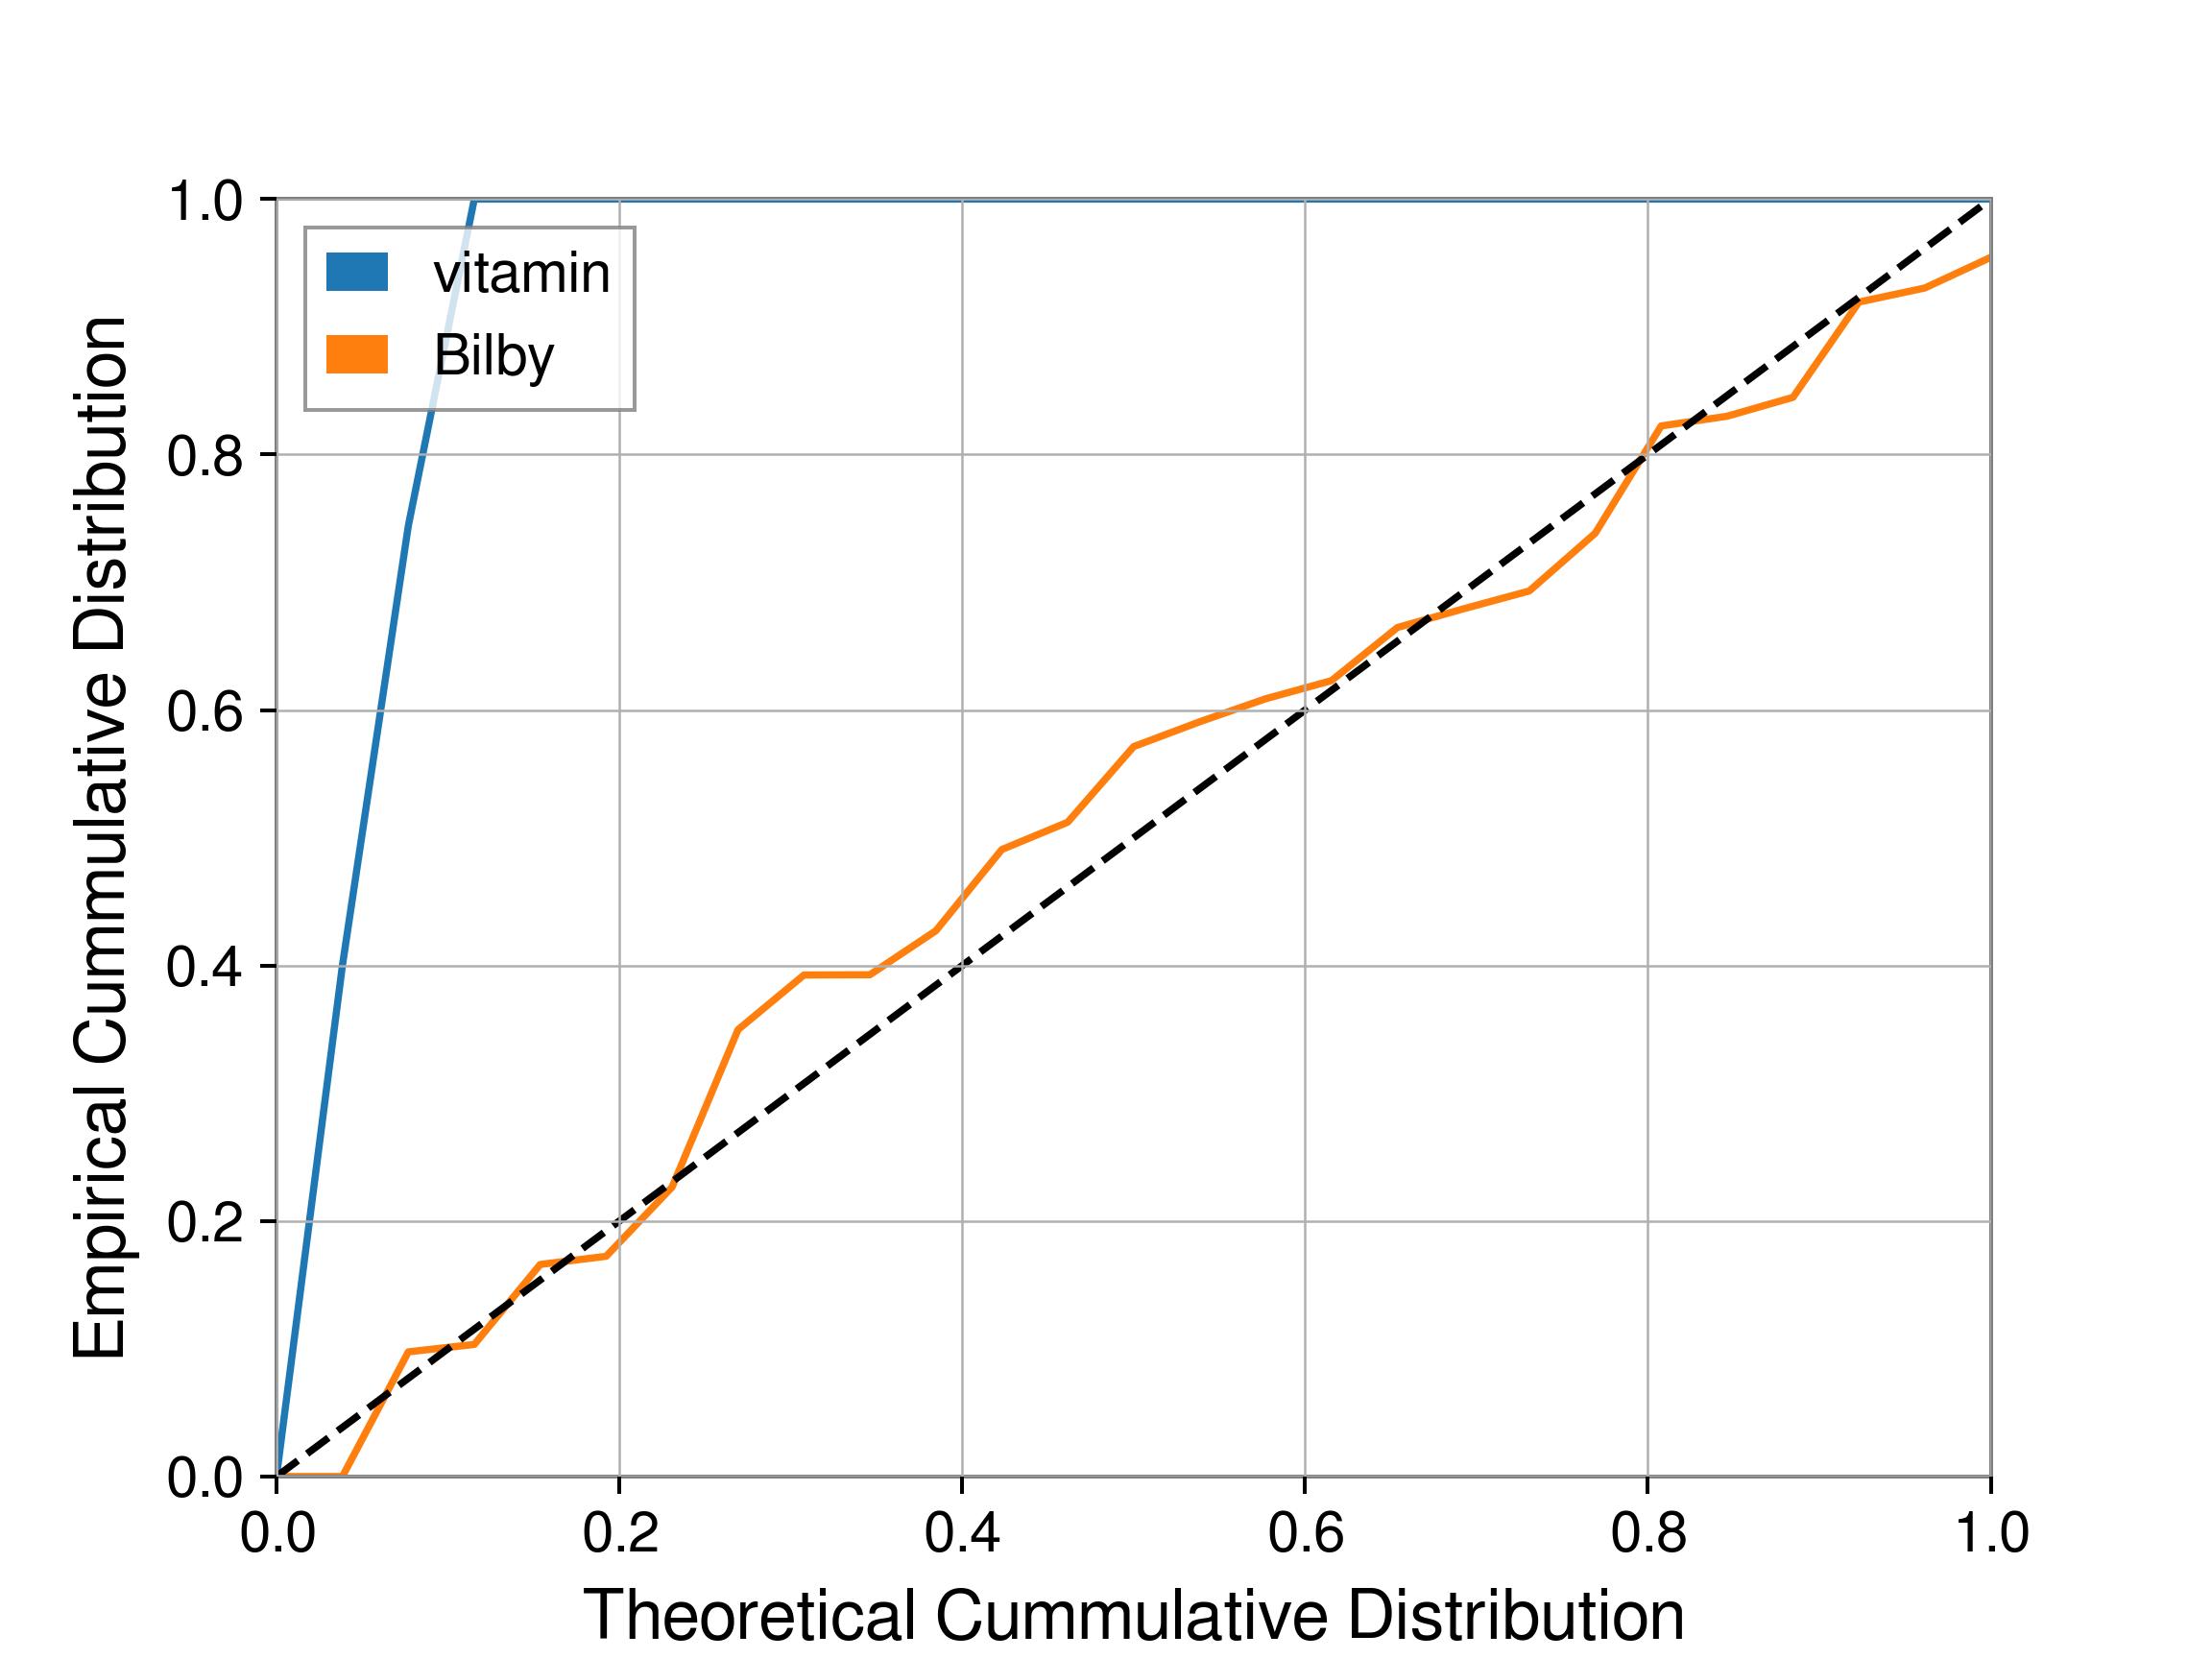
\includegraphics[width=\columnwidth]{images/latest_pp_plot.png}
    \caption{\label{fig:pp_plot} One-dimensional \ac{PP} plots for each
parameter and each benchmark sampler and \texttt{VItamin}.  The curves were
constructed using the 256 test datasets. The dashed black diagonal line
indicates the ideal result.   
}
\end{figure}
%

%
% discuss pp plot result
%
%\chris{You need to better describe what a P-P plot is and why we use it. Maybe
%throw in a reference to existing PE group papers that use it. Nature readers
%will have never seen one before. We also have to wait until we get better P-P
%plot curves for our approach before we warrant adding it to the paper.} 
A standard test used within the \ac{GW} parameter estimation community is the
production of so-called \ac{PP} plots which we show for our analysis in
Fig.~\ref{fig:pp_plot}. The plot is constructed by computing a p-value for each
output test posterior on a particular parameter evaluated at the true
simulation parameter value (the fraction of posterior samples $>$ the
simulation value). We then plot the cumulative distribution of these
values~\cite{1409.7215}. Curves consistent with the black dashed diagonal line
indicate that the 1-dimensional Bayesian probability distributions are
consistent with the frequentist interpretation - that the truth will lie within
an interval containing $X\%$ of the posterior probability with a frequency of
$X\%$ of the time. It is clear to see that our new approach shows deviations
from the diagonal that are entirely consistent with those observed in all
benchmark samplers. In Fig.~\ref{fig:kl_results} (see Sec.~\ref{sec:methods})
we also show distributions of the \ac{KL} divergence statistic between all
samplers on the joint posterior distributions. It is also clear that the
\ac{KL} divergences between \texttt{VItamin} and any other sampler are
consistent with the distributions between any 2 existing benchmark samplers.      

%
% discuss the speed of the analysis
%
The dominating computational cost of running \texttt{VItamin} lies in the
training time, which can take of order several hours to complete.  Completion
is determined by comparing posteriors produced by the machine learning model
and those of \texttt{Bilby} iteratively during training. We additionally assess
whether the cost curves (Fig.~\ref{fig:loss_log}) have converged, such that 
their slope is near-zero. We use a 
single Nvidia Tesla V100 \acp{GPU} with $16/32$ Gb of RAM although home-use
"gaming" \ac{GPU} cards are equally fast for this application. 

We stress that
once trained, there is no need to retrain the network unless the user wishes to
use different priors $p(x)$ or assume different noise characteristics.   The
speed at which posterior samples are generated for all samplers used, including
\texttt{VItamin}, is shown in Table~\ref{Tab:speed}. Run-time for the benchmark
samplers is defined as the time to complete their analyses when configured
using their default parameters~\cite{1811.02042}. For \texttt{VItamin} this
time is defined as the total time to produce $3000$ samples. For our test case
of \ac{BBH} signals \texttt{VItamin} produces samples from the posterior at a
rate which is $\sim 6$---$7$ orders of magnitude faster than current inference
techniques, representing a dramatic speed-up in performance. 

%\chris{One more thing to add, especially if the other KL, AD, and PP plots
%aren't convincing, is a plot displaying 1D confidence bounds compared between
%bilby and VItamin. Imagine a plot with the x-axis as distance and the y-axis
%steps through test data with increasing true distance. for each test data you
%plot 2 error bars horizontally (one for bilby and one for VItamin) spanning the
%range of 90\% confidence. You would hopefully get nearly identical pairs of
%errorbars stacked vertically. Technically you could do this for all parameters
%(and you should) but we might only put one of the plots in the paper (if at
%all).}

%
% I feel the need, the need for speed, table
% 
\begin{table}
\centering
\caption{Durations required to produce samples from each of
the different posterior sampling approaches.}
\begin{tabular}[t]{lcccc}
\toprule
\multirow{2}{*}{sampler} & \multicolumn{3}{c}{run time (seconds)} & \multirow{2}{*}{ratio
$\displaystyle\frac{\tau_{\text{VItamin}}}{\tau_{X}}$} \\
& min & max & median & \\
\hline
Dynesty\footnote{The benchmark samplers all produced $\mathcal{O}(3000-
10000)$ samples dependent on the default sampling parameters used.} & 602 & 1538 & 774 & $2.6\times 10^{-6}$ \\
Emcee & 2005 & 11927 & 4351 & $4.6\times 10^{-7}$ \\
Ptemcee & 3354 & 12771 & 4982 & $4.0\times 10^{-7}$ \\
Cpnest & 1431 & 5405 & 2287 & $8.8\times 10^{-7}$ \\
\texttt{VItamin}\footnote{For the \texttt{VItamin} sampler $3000$ samples are
produced as representative of a typical posterior. The run time is independent
of the signal content in the data and is therefore constant for all test cases.} & \multicolumn{3}{c}{\bm{$2\times 10^{-3}$}} & 1 \\
\botrule
\end{tabular}
\label{Tab:speed}
\end{table}

%
% word count ~960 - approx 9.6 words per line
%

%%%%%%%%%%%%%%%%%%%%%%%%%%%%%%%%%%%%%%%%%%%%%%%%%%%%%%%%%%%%%%%%%%%%%%
% CONCLUSIONS
%%%%%%%%%%%%%%%%%%%%%%%%%%%%%%%%%%%%%%%%%%%%%%%%%%%%%%%%%%%%%%%%%%%%%%
%
% conclusions - now draw conclusions about the quality of the comparison
% results. Highlight the current limitations but also highlight the importance of
% this for the GW field (multi-detector is easy, additional parameters are easy,
% longer datasets may be a challenge regarding GPU memory?, we don't have to
% assume a noise model if we inject training data into real noise, we do rely on
% well defined signal models, EM-follow up in very low latency, can we use
% transfer learning if we want to retrain, ...) End with broader statements about
% inference in other fields and how this is applicable across the sciences.
%
% recap and main result
%
In this letter we have demonstrated that we are able to reproduce, to a high
degree of accuracy, Bayesian posterior probability distributions generated
through machine learning. This is accomplished using \acp{CVAE} trained on
simulated \ac{GW} signals and does not require the input of precomputed
posterior estimates. We have demonstrated that our neural network model which,
when trained, can reproduce complete and accurate posterior estimates in
$\mathcal{O}(1)$ millisecond, can achieve the same quality of results as the
trusted benchmark analyses used within the LIGO-Virgo Collaboration.

%
% CBC implications and why this is a game-changer - speed for EM followup
%
The significance of our results is most evident in the orders of magnitude
increase in speed over existing approaches. This will help the
LIGO-Virgo collaboration alert \ac{EM} follow-up partners with minimum latency, 
enabling tightly coupled, closed-loop control of sensing resources, for maximum information gain.
Improved low-latency alerts will be especially pertinent for signals from
\ac{BNS} mergers (e.g. GW170817~\cite{PhysRevLett.119.161101}) and \ac{NSBH} signals where
parameter estimation speed will no longer be limiting factor\footnote{The complete
low-latency pipeline includes a number of steps. The process of \ac{GW} data
acquisition is followed by the transfer of data. There is then the corresponding
analysis and the subsequent communication of results to the \ac{EM} astronomy
community after which there are physical aspects such as slewing observing
instruments to the correct pointing.} in observing the prompt \ac{EM} emission
expected on shorter time scales than is achievable with existing \ac{LVC}
analysis tools such as Bayestar~\cite{2016PhRvD..93b4013S}.

%
% CBC implications and why this is a game-changer - faster, modular
%
The predicted number of future detections of \ac{BNS} mergers ($\sim
180$~\cite{1304.0670,1811.12907}) will severely strain the \ac{GW} community's
current computational resources using existing Bayesian methods. Future
iterations of our approach will provide full-parameter estimation on \ac{CBC}
signals in $<1$ second on a single \ac{GPU}. Our trained network is also modular, and can be shared and used easily by any user to produce
results. The specific analysis described in the letter assumes a uniform prior
on the signal parameters. However, this is a choice and the network can be
trained with any prior the user demands, or users can cheaply resample
accordingly from the output of the network trained on the uniform prior. We
also note that our method will be invaluable for population studies since
populations may now be generated and analysed in a full-Bayesian manner on a
vastly reduced time scale. 

%
% future work, current limitations and prospects
%
For \ac{BBH} signals, \ac{GW} data is usually sampled at $1$---$4$ kHz
dependent upon the mass of binary. We have chosen to use the noticeably low
sampling rate of 256Hz and a single detector configuration largely in order to
decrease the computational time required to develop our approach. We do not
anticipate any problems in extending our analysis to higher sampling
frequencies other than an increase in training time and a larger burden on the
\ac{GPU} memory. Our lower sampling rate naturally limited the chosen \ac{BBH}
mass parameter space to high mass signals. We similarly do not anticipate that
extending the parameter space to lower masses will lead to problems but do
expect that a larger number of training samples may be required. Future work
will incorporate a multi-detector configuration at which point parameter
estimation will be extended to sky localisation. 

%
% Non gaussian noise and the final statement
%
In reality, \ac{GW} detectors are affected by non-Gaussian noise artefacts and
time-dependent variation in the detector noise \ac{PSD}. Existing methods
incorporate a parameterised \ac{PSD} estimation into their
inference~\cite{2015PhRvD..91h4034L}. To account for these within our scheme,
we would retrain our network at regular intervals using samples of real
detector noise (preferably recent examples to best reflect the state of the
detectors). Our work can naturally be extended to include the full range of
\ac{CBC} signal types but also to any and all other parameterised \ac{GW}
signals and to analyses of \ac{GW} data beyond that of ground based
experiments. Given the abundant benefits of this method, we hope that a variant
of this of approach will form the basis for future \ac{GW} parameter
estimation.
%
% word count ~620
%

%
% acknowledge people and funding agencies
%
\section{Acknowledgements.}
%
We would like to acknowledge valuable input from the LIGO-Virgo Collaboration,
specifically from Will Farr and the parameter estimation and machine-learning
working groups. We would additionally like to thank Szabi Marka for posing this
challenge to us. We thank Nvidia for the generous donation of a Tesla V-100 GPU
used in addition to \ac{LVC} computational resources. The authors also
gratefully acknowledge the Science and Technology Facilities Council of the
United Kingdom. CM and SH are supported by the Science and Technology Research
Council (grant No.~ST/~L000946/1) and the European Cooperation in Science and
Technology (COST) action CA17137. FT acknowledges support from Amazon Research and 
EPSRC grant EP/M01326X/1, and RM-S EPSRC grants EP/M01326X/1 and EP/R018634/1. 

%
% word count 80 
%


%% Here is the endmatter stuff: Supplementary Info, etc.
%% Use \item's to separate, default label is "Acknowledgements"

\section{addendum}
 \subsection{Competing Interests} 
    The authors declare that they have no competing financial interests.
 \subsection{Correspondence} Correspondence and requests for materials should be addressed to Hunter Gabbard~(email: h.gabbard.1@research.gla.ac.uk).

%%%%%%%%%%%%%%%%%%%%%%%%%%%%%%%%%%%%%%%%%%%%%%%%%%%%%%%%%%%%%%%%%%%%%%
% METHODS
%%%%%%%%%%%%%%%%%%%%%%%%%%%%%%%%%%%%%%%%%%%%%%%%%%%%%%%%%%%%%%%%%%%%%%
%
% methods - Everything that we couldn't fit in. Mostly validation plots.
%
\section{Methods}\label{sec:methods}
%
%Put methods in here.  If you are going to subsection it, use
%\verb|\subsection| commands.  Methods section should be less than
%800 words and if it is less than 200 words, it can be incorporated
%into the main text.

%
% What is an autoencoder?
%
Conditional variational autoencoders are a form of variational autoencoder
which are conditioned on an observation, where in our case the observation is a
1-dimensional \ac{GW} time series signal $y$. The autoencoders from which
variational autoencoders are derived are typically used for problems involving
image reconstruction and/or dimensionality reduction. They perform a regression
task whereby the autoencoder attempts to predict its own given input (model the
identity function) through a ``bottleneck layer'', a limited  and therefore distilled representation of
the input parameter space. An autoencoder is composed of two neural networks,
an encoder and a decoder~\cite{gallinari1987memoires}. %\cite{LIOU20083150}. 
The encoder network takes as
input a vector, where the number of dimensions is a fixed number predefined by
the user. The encoder converts the input vector into a (typically) lower
dimensional space, referred to as the {\it{latent space}}. A representation of
the data in the latent space is passed to the decoder network which generates a
reconstruction of the original input data to the encoder network. Through
training, the two sub-networks learn how to efficiently represent a dataset
within a lower dimensional latent space which will take on the most important
properties of the input training data. In this way, the data can be compressed
with little loss of fidelity. Additionally, the decoder simultaneously learns
to decode the latent space representation and reconstruct that data back to its
original form (the input data).

%
% What is a variational autoencoder?
%
The primary difference between a variational autoencoder~\cite{1812.04405} and
an autoencoder concerns the method by which locations within the latent space
are produced. In our variant of the variational autoencoder, the output of the
encoder is interpreted as a set of parameters governing statistical
distributions (in our case the means and variances of multivariate Gaussians).
In proceeding to the decoder network, samples from the latent space ($z$) are
randomly drawn from these distributions and fed into the decoder, therefore
adding an element of variation into the process. A particular input can then
have a range of possible outputs. In both the decoder and the encoder networks
we use fully-connected layers (although this is not a constraint and any
trainable network architecture may be used).

%%%%%%%%%%%%%%%%%%%%%%%%%%%%%%%%%%%%%%%%%%%%%%%%%%%%%%%%%%%%%%%%%%%%%%
\subsection{Cost function derivation}
%
% A description of the loss function derivation 
%
We will now derive the cost function and the corresponding network structure
and we begin with the statement defining the aim of the analysis. We wish to
obtain a function that reproduces the posterior distribution (the probability
of our physical parameters $x$ given some measured data $y$). The cross entropy
between 2 distributions is defined in Eq.~\ref{eq:cross_ent} where we have made
the distributions explicitly conditional on $y$ (our measurement). In this case
$p(x|y)$ is the target distribution (the true posterior) and $r_{\theta}(x|y)$
is the parametric distribution that we will use neural networks to construct.
The variable $\theta$ represents the trainable neural network parameters. 

The cross-entropy is minimised when $p(x|y)=r_{\theta}(x|y)$ and so by
minimising
%
\begin{align}\label{eq:cost1}
H &= -\text{E}_{p(y)}\left[\int dx\,p(x|y) \log r_{\theta}(x|y)\right],
\end{align}
% 
where $\text{E}_{p(y)}[\cdot]$ indicates the expectation value over the
distribution of measurements $y$, we therefore make the parametric distribution
as similar as possible to the target for all possible measurements $y$.

Converting the expectation value into an integral over $y$ weighted by $p(y)$
and applying Bayes' theorem we obtain
%
\begin{align}\label{eq:cost1}
H &= -\int dx\,p(x)\int dy\,p(y|x)\log r_{\theta}(x|y)
\end{align}
%
where $p(x)$ is the prior distribution on the physical parameters $x$.

The \ac{CVAE} network outlined in Fig.~\ref{fig:network_config} makes use of a
conditional latent variable model and our parametric model is constructed from
the product of 2 separate distributions marginalised over the latent space
%
\begin{align}\label{eq:latent_model}
r_{\theta}(x|y) &= \int dz\,r_{\theta_{1}}(z|y)r_{\theta_{2}}(x|z,y).
\end{align}
%  
We have used $\theta_{1}$ and $\theta_{2}$ to indicate that the 2 separate
networks modelling these distributions will be trained on these parameter sets
respectively. Both new conditional distributions are modelled as $n_{z}$
dimensional multivariate uncorrelated Gaussian distributions (governed by their
means and variances). However, this still allows $r_{\theta}(x|y)$ to take a
general form (although it does limit it to be unimodal).  

One could be forgiven in thinking that by setting up networks that simply aim
to minimise $H$ over the $\theta_{1}$ and $\theta_{2}$ would be enough to solve
this problem. However, as shown in~\cite{NIPS2015_5775} this is an intractable
problem and a network cannot be trained directly to do this. Instead we define
a recognition function $q_{\phi}(z|x,y)$ that will be used to derive an
\ac{ELBO}. Here we use $\phi$ to represent the trainable parameters of an
encoder network ($\text{E}_{2}$).

Let us first define the \ac{KL} divergence between 2 of our
distributions as
%
\begin{align}\label{eq:kl}
\text{KL}&\left[q_{\phi}(z|x,y)||r_{\theta_{2}}(z|x,y)\right] = \\
&\int dz\,q_{\phi}(z|x,y)
\log\left(\frac{q_{\phi}(z|x,y)}{r_{\theta_{2}}(z|x,y)}\right).\nonumber
\end{align}
%  
It can be shown, after some manipulation, that
%
\begin{align}\label{eq:elbo1}
\log r_{\theta}(x|y) &= L + \text{KL}\left[q_{\phi}(z|x,y)||r_{\theta_{?}}(z|x,y)\right],
\end{align}
%
where the \ac{ELBO} $L$ is given by
%
\begin{align}\label{eq:elbo2}
L &= \int dz\,
q_{\phi}(z|x,y)\log\left(\frac{r_{\theta_{2}}(x|z,y)r_{\theta_{1}}(z|y)}{q_{\phi}(z|x,y)}\right)
\end{align}
%
and is so-named since $\text{KL}$ cannot be negative and has a minimum of zero.
Therefore, if we were to find a $q_{\phi}(z|x,y)$ function (optimised on
$\phi$) that minimised the \ac{KL}-divergence then we can state that
%
\begin{align}
\log r_{\theta}(x|y) &\geq L.
\end{align}
%
After some further manipulation of Eq.~\ref{eq:elbo2} we find that
%
\begin{align}\label{eq:logr}
\log r_{\theta}(x|y) \geq  &\text{E}_{q_{\phi}(z|x,y)}\left[\log
r_{\theta_{2}}(x|z,y)\right] \nonumber\\
&-\text{KL}\left[q_{\phi}(z|x,y)||r_{\theta_{1}}(z|y)\right].
\end{align}
%
We can now substitute this inequality into Eq.~\ref{eq:cost1} (our cost
function) to obtain
%
\begin{align}\label{eq:cost2}
H \leq  -\int dx\, p(x)\int dy &\,p(y|x)
\Big[\text{E}_{q_{\phi}(z|x,y)}\left[\log r_{\theta_{2}}(x|z,y)\right]
\nonumber\\
&-\text{KL}\left[q_{\phi}(z|x,y)||r_{\theta_{1}}(z|y)\right]\Big],  
\end{align}
%
which can in practice be approximated as a stochastic integral over draws of
$x$ from the prior, $y$ from the likelihood function $p(y|x)$, and from the
recognition function, giving us Eq.~\ref{eq:cost3}, the actual function
evaluated within the training procedure.

%
% loss plot
%
\begin{figure}
    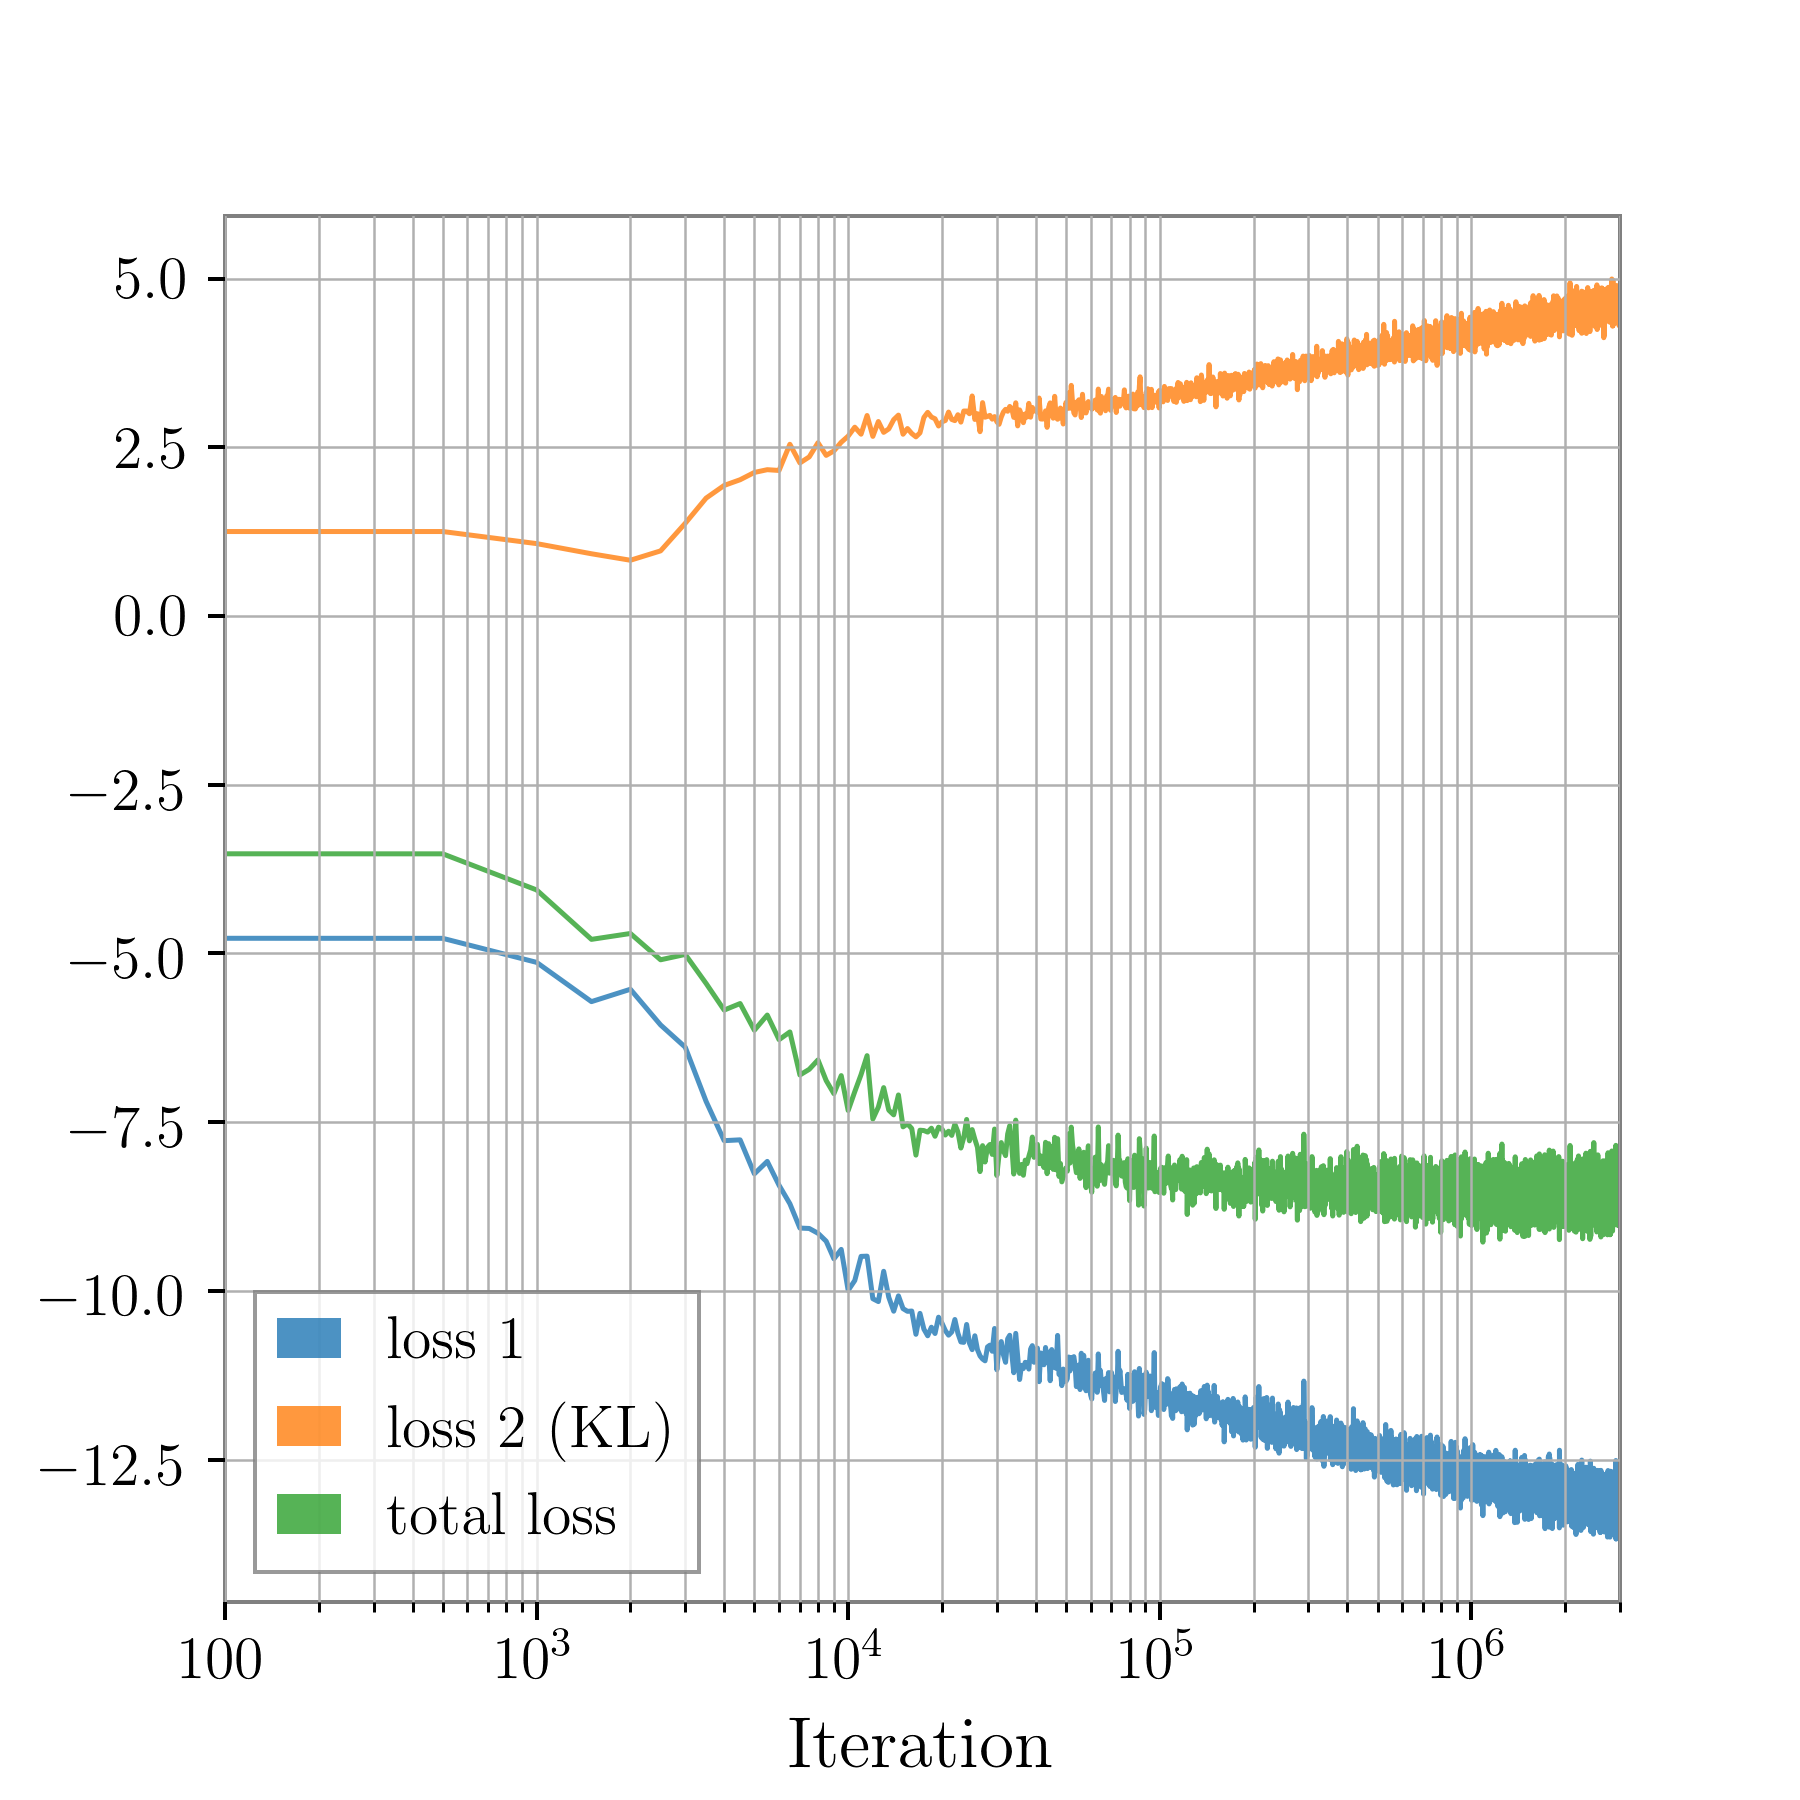
\includegraphics[width=\columnwidth]{images/inv_losses_log.png}
\caption{\label{fig:loss_log} The cost as a function of training iteration. We
show the \ac{ELBO} cost function component (blue), the \ac{KL} divergence
component (orange) and total cost (green). The total cost is simply a
summation of the 2 components and one training iteration is defined as
training over one batch of signals.}
\end{figure}

%
% Priors
%
\begin{table}
\centering
\caption{The uniform prior boundaries and fixed parameter values used on the \ac{BBH} signal parameters for the benchmark
and the \ac{CVAE} analyses.}
\begin{tabular}[t]{lcccc}
\toprule
Parameter name & symbol & min & max & units \\
\hline
mass 1 & $m_1$ & 35 & 80 & solar masses \\
mass 2 & $m_2$\footnote{Additionally $m_2$ is constrained such that
$m_{2}<m_{1}$.} & 35 & 80 & solar masses \\
luminosity distance & $d_{\text{L}}$ & 1 & 3 & Gpc \\
time of coalescence & $t_{0}$ & 0.65 & 0.85 & seconds \\
phase at coalescence & $\phi_{0}$ & 0 & $2\pi$ & radians \\
\hline
right ascension & $\alpha$ & \multicolumn{2}{c}{1.375} & radians \\
declination & $\delta$ & \multicolumn{2}{c}{-1.2108} & radians \\
inclination & $\iota$ & \multicolumn{2}{c}{0} & radians \\
polarisation & $\psi$ & \multicolumn{2}{c}{0} & radians \\
spins & - & \multicolumn{2}{c}{0} & - \\
epoch & - & \multicolumn{2}{c}{1126259642} & GPS time \\
detector & - & \multicolumn{2}{c}{H1} & - \\
\botrule
\end{tabular}
\label{tab:prior_ranges}
\end{table}

%%%%%%%%%%%%%%%%%%%%%%%%%%%%%%%%%%%%%%%%%%%%%%%%%%%%%%%%%%%%%%%%%%%%%%
\subsection{The training procedure}
%
% Introduce the training process
%
Having set up a cost function composed of 3 probability functions that have
well defined inputs and outputs where the mapping of those inputs to outputs is
governed by the parameter sets $\theta_{1},\theta_{2},\phi$. These parameters
are the weights and biases of 3 neural networks acting as (variational)
encoder, decoder, and encoder respectively. To train such a network one must
connect the inputs and outputs appropriately to compute the cost function $H$
and back-propagate cost function derivatives to update the network parameters.
The network structure shown schematically in Fig.~\ref{fig:network_config}
shows how for a batch of $N$ sets of $x$ and corresponding $y$ values, the cost
function is computed during each iteration of training. 

%
% Go through the training step by step
%
Training is performed via a series of steps illustrated in
Fig.~\ref{fig:network_config}.
%
\begin{itemize}
%
\item The encoder $\textrm{E}_1$ is given a set of training \ac{GW} signals
($y$) and encodes $y$ into a set of variables $\mu_q$ defining a distribution
in the latent space. In this case $\mu_q = (\mu_{q0},\sigma^{2}_{q})$ describes
the first 2 central moments (mean and variance) for each dimension of a
uncorrolated (diagonal covariance) multivariate Gaussian distribution.
%
\item The encoder $\textrm{E}_2$ takes a combination of both the data $y$ and
the true parameters $x$ defining the \ac{GW} signal and encodes this into
parameters defining another uncorrelated multivariate Gaussian distribution in
the same latent space. These parameters we denote by
$\mu_{r}=(\mu_{r0},\sigma^{2}_{r})$ again representing the means and variances.
%
\item We then sample from the distribution described by $\mu_{q}$ giving us
samples $z_{q}$ within the latent space.
%
\item These samples, along with their corresponding $y$ data, then go to the
decoder D which outputs $\mu_{x}=(\mu_{x0},\sigma^{2}_{q})$, a set of parameters (much like
$\mu_q,\mu_r$) that define the moments of an uncorrelated  multivariate Gaussian
distribution in the physical $x$ space.
 %
\item The first term of the loss function (Eq.~\ref{eq:cost3}) is then computed
by evaluating the probability density defined by $\mu_x$ at the true $x$
training values. The component of the loss allows the network to learn how to
predict accurate values of $x$ but to also learn the intrinsic variation due to
the noise properties of the data $y$. It is important to highlight that the
\ac{GW} parameter predictions from the decoder D do describe a multivariate
Gaussian, but as is shown in our results (see Fig.~\ref{fig:corner_plot}), this
does \emph{not} imply that our final output posterior estimates will also be
multivariate Gaussians.
%
\item Finally the loss component described by the \ac{KL} divergence between the
distributions described by $\mu^{q}$ and $\mu^{r}$ is computed using
%
\begin{align}\label{eq:klgauss}
\text{KL}&\left[q_{\phi}(z|x_{n},y_{n})||r_{\theta_{1}}(z|y_{n})\right] = \\
&\frac{1}{2}\sum_{j=1}^{n_{z}}\left[\frac{\sigma_{q,j}^{2}}{\sigma_{r,j}^{2}} +
\frac{(\mu_{r0,j}-\mu_{q0,j})^{2}}{\sigma_{r,j}^{2}}+
\log\left(\frac{\sigma_{r,j}^{2}}{\sigma_{q,j}^{2}}\right)\right] -
\frac{n_{z}}{2}.\nonumber 
\end{align}
%
Here we highlight that we do not desire that the network tries to make these 2
distributions equal to each other. Rather, we want the ensemble network to
minimise the total cost (of which this is a component).
%
\end{itemize}

%
% Some practical aspects of the training
%
As is standard practice in machine learning applications, the cost
is computed over a batch of training samples and repeated for a pre-defined
number of iterations. 


%%%%%%%%%%%%%%%%%%%%%%%%%%%%%%%%%%%%%%%%%%%%%%%%%%%%%%%%%%%%%%%%%%%%%%
\subsection{Network and Training parameters}
%
% Describe the specific network hyper-parameters
%
For our purposes, we found that $\sim3\times10^6$ training iterations, a batch
size of $512$ training samples and a learning rate of $10^{-4}$ was sufficient.
We used a total of $10^6$ training samples in order to adequately cover the
\ac{BBH} parameter space. We additionally ensure that an (effectively) infinite
number of noise realizations are employed by making sure that every time a
training sample is used it is given a unique noise realisation despite only
having a finite number of waveforms. Each neural network ($\text{E}_1$,
$\text{E}_2$, D) is composed of 3 fully connected layers and has $2048$ neurons
in each layer with ReLU~\cite{nair2010rectified} activation functions between
layers. We use a latent space dimension of $8$ and we consider training
complete when both components to the loss function have converged to
approximately constant values or when comparisons with benchmark test
posteriors indicate no significant changes in the output posterior.

%%%%%%%%%%%%%%%%%%%%%%%%%%%%%%%%%%%%%%%%%%%%%%%%%%%%%%%%%%%%%%%%%%%%%%
\subsection{The testing procedure}
%~\chris{Hunter, note that we only need to
%do the first pass through E1 only once for a given piece of data do the real
%cost is only in the other steps. This will likely only change the timing by
%~25\% so it might not be worth doing the tests again. Just bear it in mind.}
%
%
% Introduce the testing procedure
%
After training has completed and we wish to use the network for inference we
follow the procedure described in the right hand panel of
Fig.~\ref{fig:network_config}. Given a new $y$ data sample (not taken from the
training set) we simply input this into the encoder $\textrm{E}_1$ from which we
obtain a single value of $\mu_{r}$ describing a distribution (conditional on the
data $y$) in the latent space. We then repeat the following steps:

%
% Go through the testing step by step
%
\begin{itemize}
%
\item We randomly draw a latent space sample $z_r$ from the latent space
distribution defined by $\mu_r$.
%
\item Our $z_r$ sample and the corresponding original $y$ data are fed as input to our
pre-trained decoder network (D). The decoder network returns a set of moments
$\mu_{x}$ which describe a multivariate Gaussian distribution in the physical
parameter space.
%
\item We then draw a random $x$ realisation from that distribution.
%
\end{itemize}
%

%
% Final testing thoughts
%
A comprehensive representation in the form of samples drawn from the entire joint
posterior distribution can then be obtained by simply repeating this procedure
with the same input data (see Eq.~\ref{eq:latent_model}).

%
% K-L divergence results
%
\subsection{Additional tests}
%
\begin{figure}
    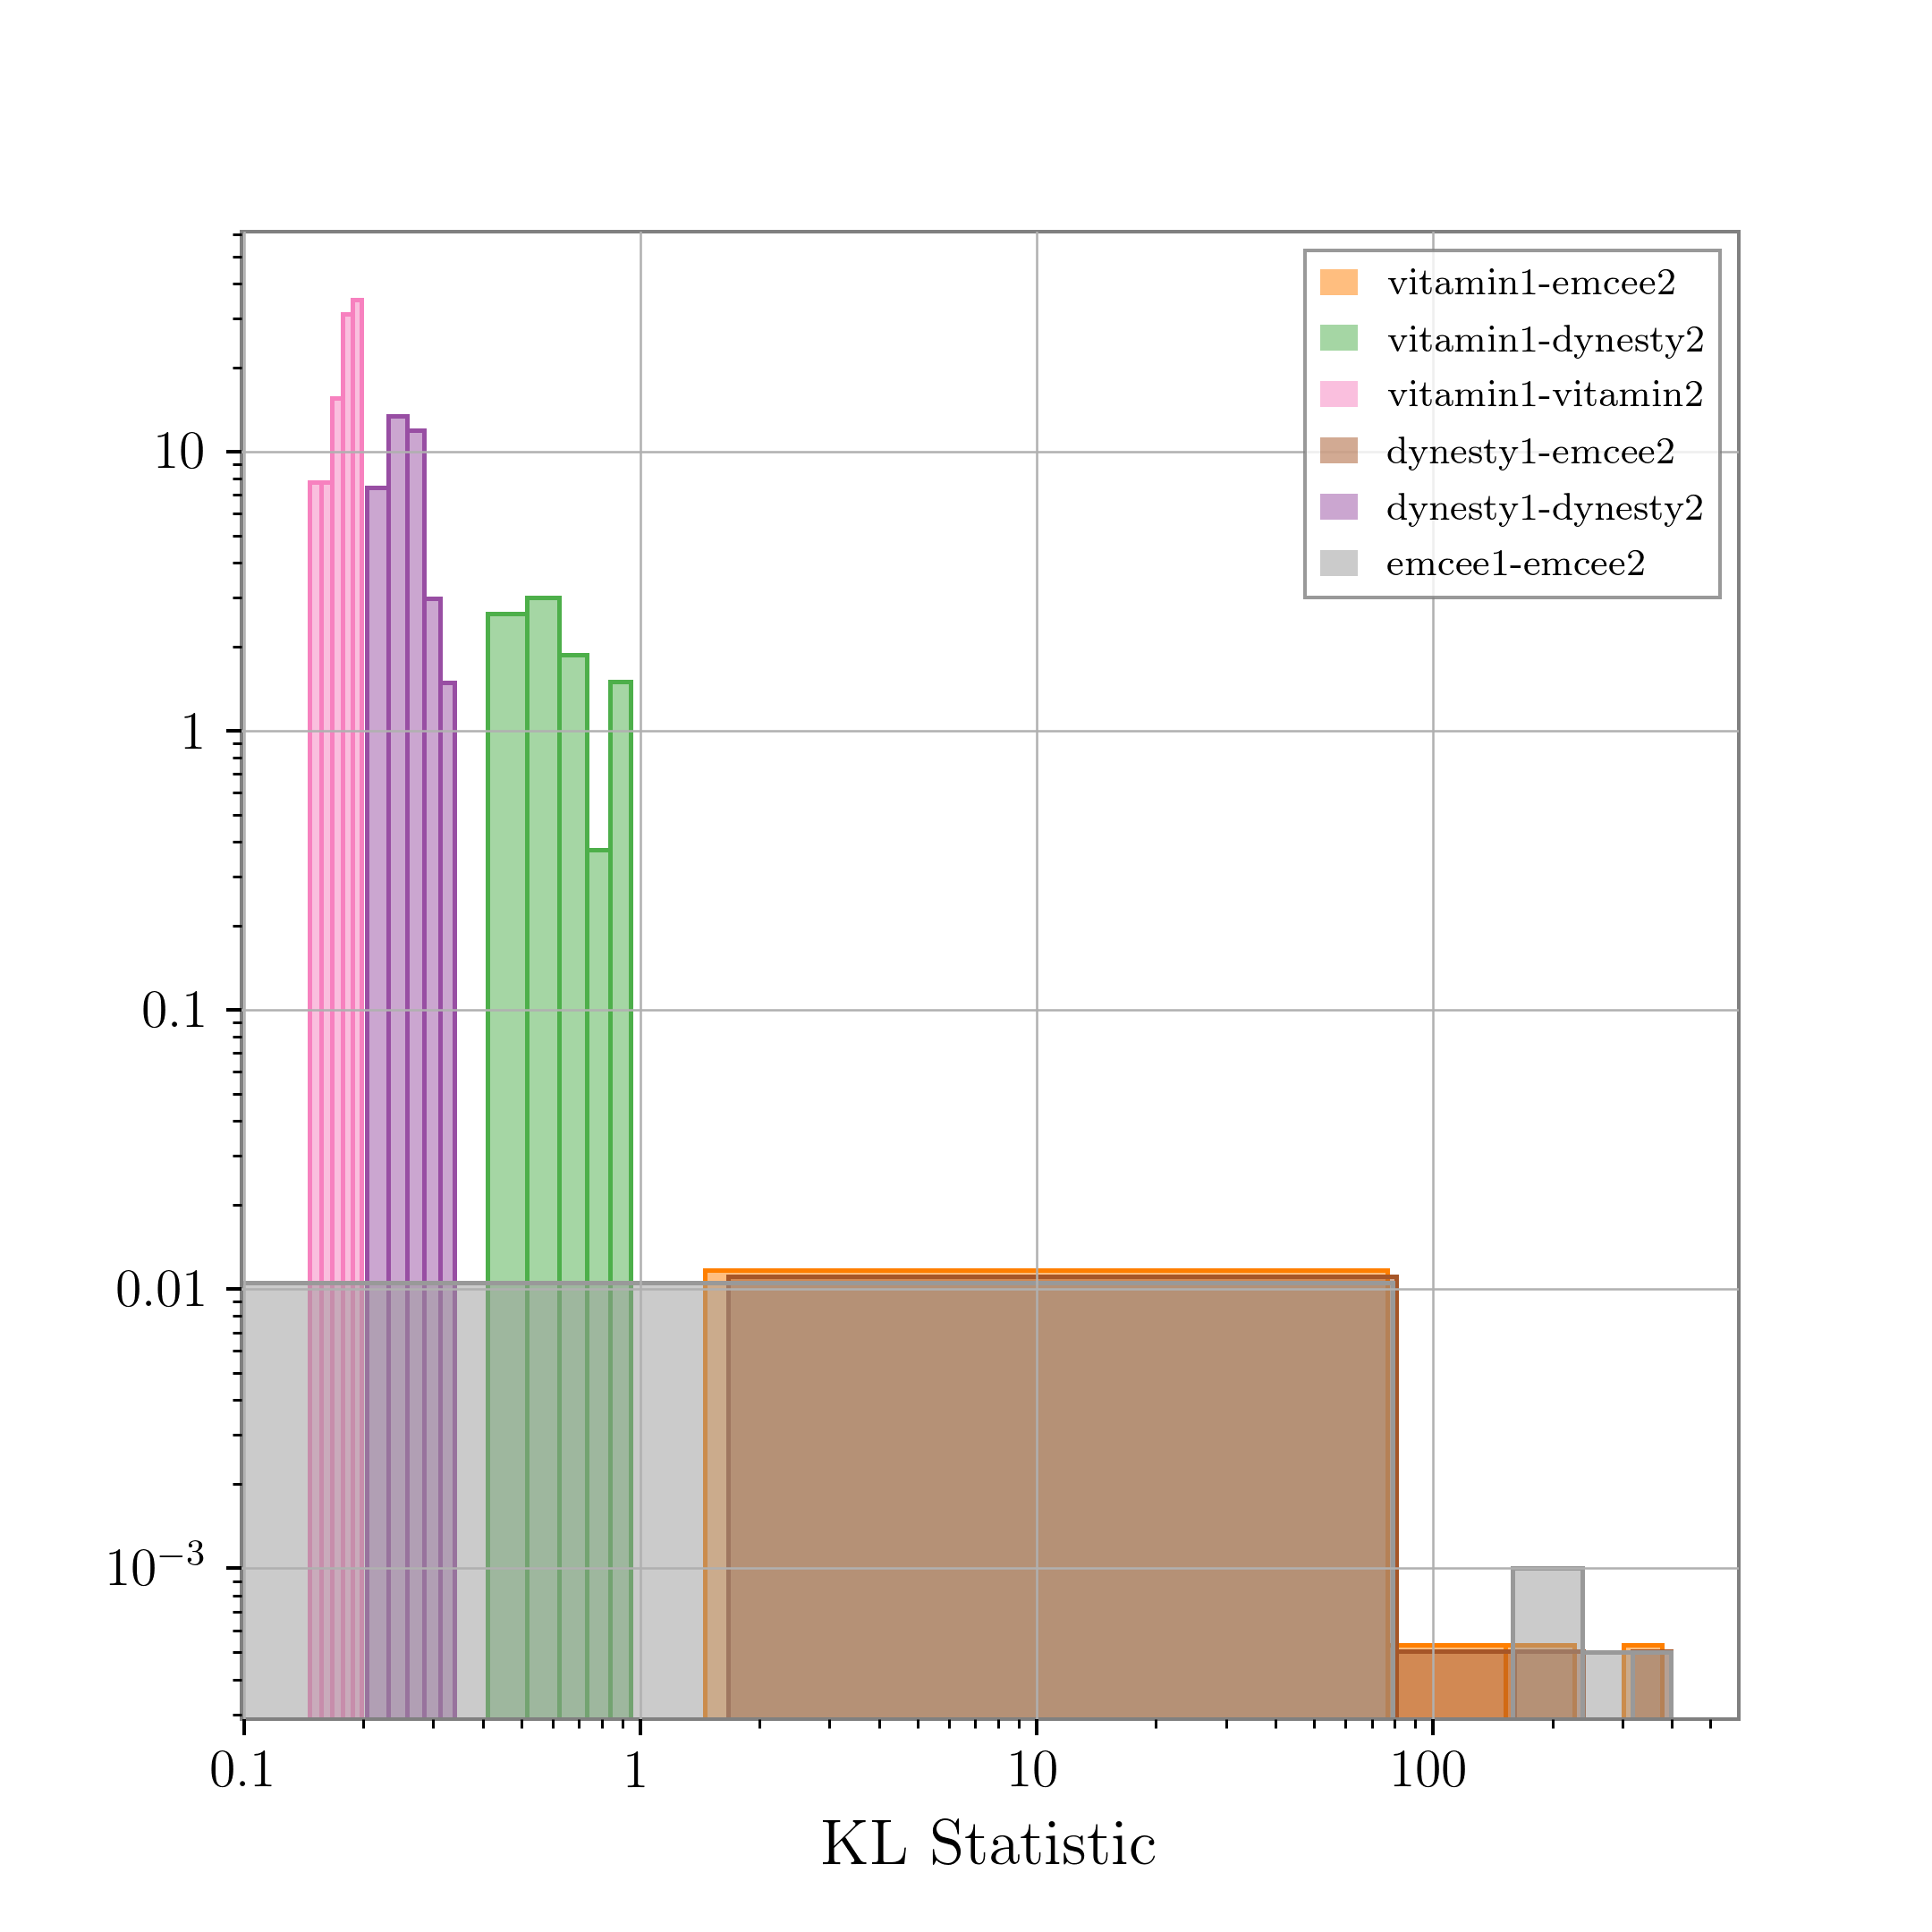
\includegraphics[width=\columnwidth]{images/hist-kl.png}
    \caption{\label{fig:kl_results} Distributions of \ac{KL}-divergence values
between posteriors produced by different samplers. The \ac{KL} divergence is
computed between all samplers with every other sampler over all 256 \ac{GW}
test cases. The distributions of the resulting \ac{KL} divergence values are
then plotted, with each color representing a different sampler combination
including \texttt{VItamin} as one of the sampler pairs. The grey distributions
represent the results from all benchmark sampler pairs for comparison. Both the
$x$ and $y$ axes are scaled logarithmically for readability.} 
\end{figure}
%

%
% discuss the KL results
%
The \ac{KL} divergence between 2 distributions is a measure of their similarity
and we use this to compare the output posterior estimates between samplers for
the same input test data. To do this we run each independent sampler (including
the \ac{CVAE}) on the same test data to produce samples from the corresponding
posterior. We then compute the \ac{KL}-divergence between output distributions
from each sampler with itself and each sampler with all other samplers. For
distributions that are identical the \ac{KL}-divergence is equal to zero but
since we are representing our posterior distributions using finite numbers of
samples, identical distributions should result in KL-divergence values $<1$. In
Fig.~\ref{fig:kl_results} we show the distributions of these
\ac{KL}-divergences for the 256 test \ac{GW} samples where we see that the
\ac{CVAE} approach when compared to the benchmark samplers have distributions
consistent with those produced when comparing between 2 different benchmark
samplers.

\bibliographystyle{apsrev4-1}
\bibliography{references}% Produces the bibliography via BibTeX.

\end{document}
